\documentclass[12pt, letterpaper]{elsarticle}
\usepackage[utf8]{inputenc}
\usepackage{graphicx}
\usepackage{siunitx}
\usepackage{multirow}
\usepackage{subcaption}

\title{Neutronics Aspects of the FESS-FNSF}
\author[wisc]{A. Davis\corref{cor1}}
\ead{andrew.davis@wisc.edu}
\author[wisc]{M. Harb}
\ead{mharb@wisc.edu}
\author[wisc]{L. El-Guebaly}
\ead{elguebaly@wisc.edu}
\author[wisc]{P. Wilson}
\ead{paul.wilson@wisc.edu}
\author[wisc]{E. Marriott}
\ead{marriott@wisc.edu}
\author{FESS-FNSF team}
\ead[url]{http://cnerg.wisc.edu}
\cortext[cor1]{Corresponding author}

\address[wisc]{The University of Wisconsin-Madison, Deparment of Engineering Physics, 1500 Engineering Drive, Madison, WI 53706}
 
\begin{document}
 
\begin{abstract}
Neutronics analysis was performed on the latest Fusion Energy System Studies - Fusion Nuclear Science Facility (FESS-FNSF) design, which determined the neutron wall loading, tritium breeding ratio, and radiation damage. Sixteen different sectors configurations were investigated, with the main focus on determining the impact which each has upon the tritium breeding ratio (TBR) of the whole facility. This paper describes the stages of the nuclear analysis that serve to prove the radiation derived attributes of the system.

\vspace{5mm}
\noindent
Keywords: FESS-FNSF, tritium breeding ratio, radiation damage, DAGMC
\end{abstract}

\begin{titlepage}
\maketitle
\end{titlepage}

\newpage
\listoffigures

\newpage
\section{Introduction} \label{Introduction}
The Fusion Energy Systems Studies - Fusion Nuclear Science Facility (FESS-FNSF \cite{ref_1}) is considered an essential element of the US fusion road map that displays a strategic pathway from ITER to a US DEMO, and eventually to the first commercial power plant. A FNSF will help bridge the research gap between ITER - low radiation damage, short pulses, no significant tritium breeding - and DEMO which is designed to operate at power plant relevant fusion parameters. The FNSF will advance the understanding of fusion nuclear sciences (FNS) by providing an integrated platform for establishment of a database on all components. These components will be irradiated up to relevant parameters (e.g. 40-60 dpa, blanket temperatures 500-600\textsuperscript{o}C) via in-depth investigation of issues related to plasma boundary interface (materials interaction with high energy neutron flux, surface/volumetric heating, radiation damage, and gas production), operating in power plant relevant fusion core conditions (temperatures, coolant/breeder flow rates, pressures/stresses, B-field, and neutrons), tritium breeding/extraction/processing, advancing and demonstrating plasma technologies that support very long duration operations, etc.\vspace{5mm}

The FNSF subjected to this study is a tokamak-based facility with a \SI{518}{MW} fusion power, a plant Lifetime of $\sim$ \SI{24}{years} ($\sim$ \SI{8.5}{FPY}) and $\sim 35\%$ availability. The machine average neutron wall loading (NWL) at the first wall is \SI{1.1}{MW/m\textsuperscript{2}}. The radiation damage to the first wall was calculated followed by a shielding analysis. Shielding optimisation \cite{ref_2} involved testing the effect of the inboard shielding materials on the radiation damage levels at the magnet with an inboard breeding blanket and the results showed that the radiation levels at the magnet are within acceptable limits. Such calculations involved estimating the fast neutron fluence, nuclear heating at the coil case, and atomic displacement to the Cu stabilizer. A detailed tritium breeding study was also performed to assess the effect of various design elements on the tritium breeding ratio (TBR) of the dual-cooled lithium lead (DCLL) blanket which confirmed tritium self-sufficiency, a value of TBR $\sim$ 1 with 4\% margin. In section (\ref{Analysis Tools}) the software tools used in this study will be described and in section (\ref{Neutron Wall Loading}) NWL results will be introduced. In section (\ref{Tritium Breeding Calculations}) focus will be on the tritium breeding calculations. Finally, in section (\ref{Radiation Damage}), the magnet shielding and radiation damage calculations will be discussed.

\subsection{Configuration} \label{Configuration}
The first step in the analysis involved optimisation of the Outboard (OB) \& Inboard (IB) radial builds and the divertor vertical build \cite{ref_2}. The result of such 1-D extensive optimisation analysis is a complete definition of the material composition of the different regions taking into account the configuration of the facility, radiation limits especially at the magnet (and other long lifetime components), selection of low activation materials, environmental and safety constraints, and temperature limits for several in-vessel components. Some design parameters were pre-set based on decisions made during previous studies such as ARIES-ACT2 \cite{ref_3}. Such parameters included the sizes of the He-cooled \SI{20}{cm} thick Structural Ring (SR) and \SI{10}{cm} thick Vacuum Vessel (VV) (both of these structures are composed to 2 face sheets with internal ribs and filler materials). As will be discussed in section (\ref{Radiation Damage}) the most important parameters in the analysis were the fast neutron fluence and nuclear heating at the toroidal field magnet. The OB radial build and the corresponding material composition of each layer is shown in figure \ref{fig:radial build} and the detailed composition of the OB is;
\begin{figure}[h!]
  \centering
  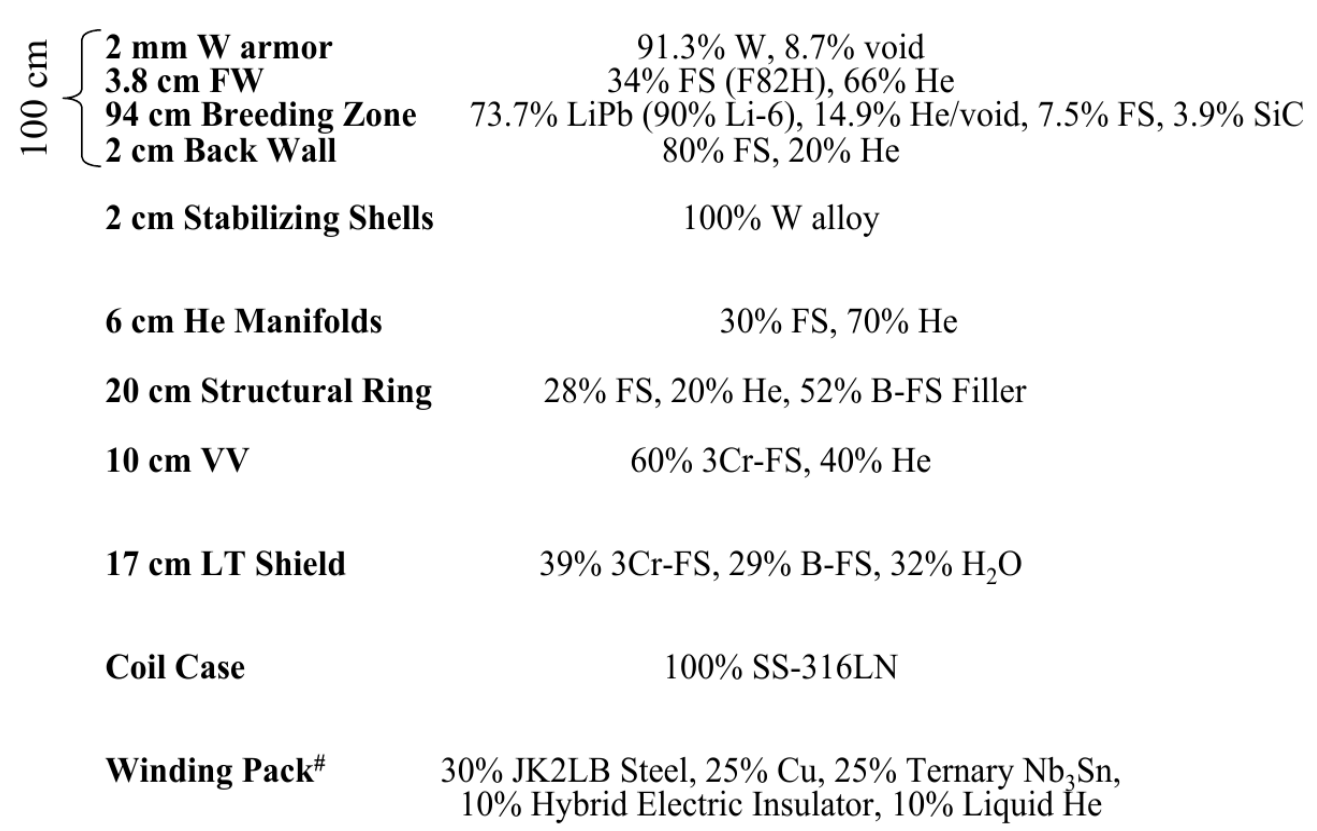
\includegraphics[scale=0.2]{../plots/OB_comp.png}
  \label{fig:OB_comp}
\end{figure}
\begin{figure}[h!]
  \centering
  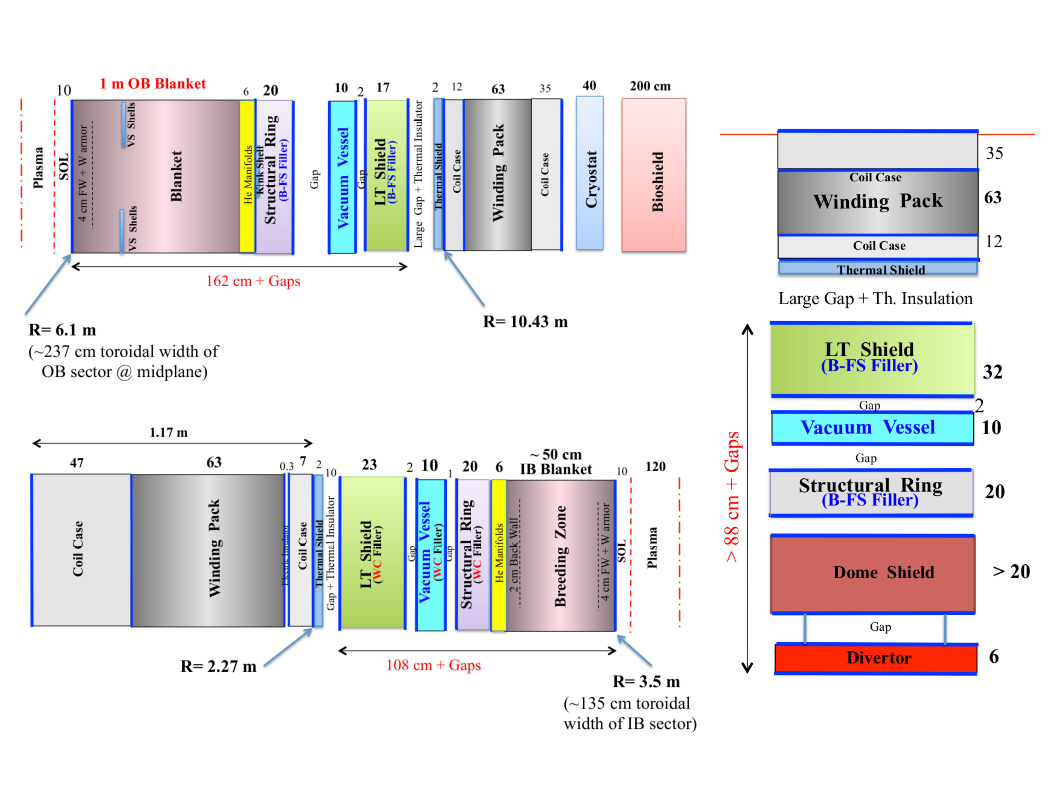
\includegraphics[scale=0.4]{../plots/radial_build.png}
  \caption{OB "top left", IB "bottom left", and Divertor "right" radial builds}
  \label{fig:radial build}
\end{figure}
\subsection{1-D Optimisation}
\label{Optimisation}
\subsubsection{Heat load to Coils}
All components should, to some degree, provide shielding function to help the device satisfy the radiation limits. In the case of the FNSF, a common filler material can be used in the Structual Ring (SR), the Vaccum Vessel (VV) and the Low Temperature (LT) shield. Several candidate filler materials have been identified: MF82H (Modified Ferritic Steel), B-FS (Borated Ferritic Steel), and WC (Tungsten Carbide). Comparison was made based on the basis of several key magnet system requirements:
\begin{itemize}
  \item{Peak nuclear heating at the winding pack ($<$ 1 mW/cm$^3$)}
  \item{Peak nuclear heating at the coil case ($<$ 2 mW/cm$^3$)}
  \item{Peak dpa to Cu stabilizer ($<$ 10$^{-4}$ dpa)}
  \item{Peak dose to electric insulator ($<$ 5$\times$10$^{10}$ rads)}
  \item{Peak fast neutron fluence to ternary Nb$_3$Sn super conductor ($<$ 3$\times$10$^{18}$ n/cm$^2$).}
\end{itemize}
2Nuclear heat deposition in Superconducting (SC) magnets is particularly problematic due to the increased probability of a quench. The cooling system is designed to remove this, however, increased cooling requirements impact the economics and superconductor design as a result of temperature change, thus heat to magnets must be minimised. The results of the optimisation calculations are shown in Table \ref{tab:1dcalc}.
\begin{table}[ht!]
 \begin{tabular}{| l | c | c | c |} 
 \hline 
 Material & MF82H & B-FS & WC \\
 \hline
 Peak Nuclear Heating at WP (mW) & 1000 & 210 & 0.3 \\
 Dose to electrical insulator (rads) & 2.5$\times$10$^5$ & 1.0$\times$10$^5$ & 190 \\
 Peak DPA to Cu stabilizer & 1.5$\times$10$^{-3}$ & 9.5$\times$10$^{-4}$ & 1.5$\times$10$^{-6}$ \\
 Peak nuclear heating at CC (mW) & 900 & 200 & 1.6 \\
 Peak fast neutron fluence to Nb$_3$Sn (n/cm$^2$s) & 4.2$\times$10$^{19}$ & 2.4$\times$10$^{19}$ & 2.0$\times$10$^{18}$ \\ 
 \hline
 \end{tabular}
 \caption{Nuclear parameters of the SC magnets as a function of filler material at 8.5 FPY}
 \label{tab:1dcalc}
\end{table}

The magnet damage reaches its minimum when WC is used as filler in SR, VV, and LT shield. WC has the ability to reduce the magnet heating, insulator dose, DPA to Cu stabilizer, and fluence by almost 90-95\% compared to other fillers, furthermore, WC has high attenuation and is endowed with several superior mechanical and thermal properties.

\subsubsection{Radiation Damage to LT Shield}
The FW and Blanket are sacrificial components that are planned to be replaced every few years due to radiation damage considerations. The LT shield helps to protect external components. Being the closest component to the SC magnets, the composition of LT shield helps to influence the radiation damage at the magnet. The LT shield is composed of H$_2$O-WC mixture. Optimisation of the composition of the LT Shield will help the design meet the FNSF radiation limits.

\begin{figure}[h!]
  \centering
  \includegraphics[scale=0.5]{../plots/fast_fluence_lt.png}
  \caption{Sensitivity of peak radiation effects at magnet to LT shield material composition}
  \label{fig:fast_fluence}
\end{figure}

It was found that the fast neutron fluence is minimised when the LT shield composition is 50\% WC and 45\% H$_2$O, an example of the optimisation results are shown in Figure \ref{fig:fast_fluence}. The nuclear heating at the coil case and winding pack minimises at higher WC content than 50\%, thus the selection of 50\% WC is slightly inoptimal. The dose to electric insulator and dpa to Cu stabilizer are found to be well below their respective limits at a composition of 50\% WC and 45\% H$_2$O. Therefore, the shield composition should have water comprising 45\% of volume and WC is 50\%, with the remaining 5\% left as FS-3Cr steel structural material. 

\subsection{Full 3D Build} \label{Full 3D Build}
The shielding and blanket optimisation described in subsection (\ref{Configuration} \& \ref{Optimisation}) resulted in a full definition of the major materials and dimensions that were used to produce the 3D assembly CAD model. Shown in Figure \ref{fig:Full3D} is a cross section of one sector with the major regions identified on the figure. The model consists of 16 IB and OB sectors with \SI{2}{cm} assembly gaps which was used in all analyses performed in this study. At full power, these gaps will close to some degree, however future designs will include some labyrinth to mitigate these effects. The facility has a major radius of \SI{4.8}{m} and a minor radius of \SI{1.2}{m}. It's worth mentioning that the CAD used in the analysis included all in-vessel components up to the IB magnet and out-of-vessel components up to the LT shield. 
\begin{figure}[h!]
  \centering
  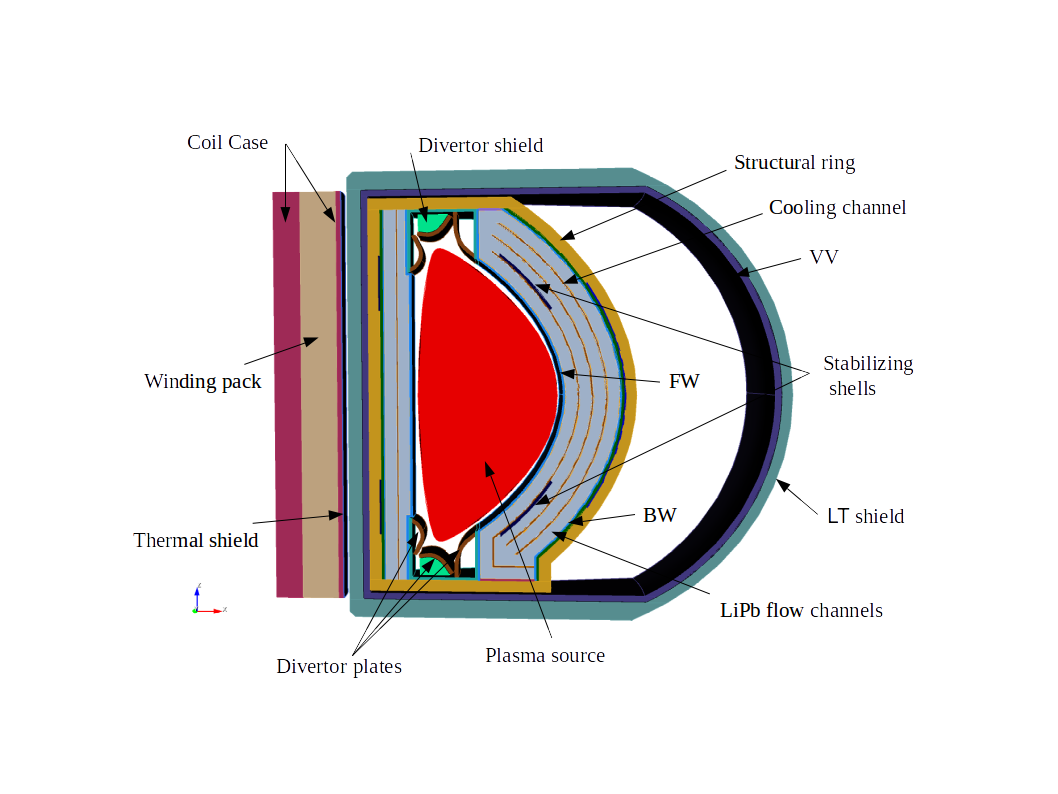
\includegraphics[scale=0.35,clip]{../plots/full_3d.png}
  \caption{The full 3D CAD model of a single FESS-FNSF sector}
  \label{fig:Full3D}
\end{figure}

\section{Analysis Tools} \label{Analysis Tools}
As will be discussed in section (\ref{Tritium Breeding Calculations}), calculation of the TBR with high fidelity has to be achieved in order to confirm the adequacy of the configuration of the facility for tritium self-sufficiency. Based on previous analyses, some margins are considered in the design phase such that the final integration of all engineering systems in the facility will ensure a TBR $>$ 1. One of the margins \cite{ref_3} considered in the design phase of the facility is directly related to deficiencies in modelling resulting from approximations introduced to facilitate the analysis especially the neutron/photon transport calculations. \vspace{5mm}

In this study the approximations were limited and only applied to design details which are known – based on accumulated experience with previous models - to be of less importance regarding neutron/photon transport calculations besides slowing down the simulations if included. Such design details include; the detailed structure of the First Wall (FW) and its He cooling system, the internal structure of the blanket cooling channels, and the internal structure of the He manifolds. Those regions are known to show little/no difference if modelled in detail or homogenized with a proper assignment of volume averaged material compositions.\vspace{5mm}

State-of-the-art analysis tools were utilized in this study which enabled working with the full 3-D model with all the internal details defined in the CAD, such as blanket internals and side/back/front walls, which are known to play a key role in TBR degradation. This work was performed with DAG-MCNP5, a version of MCNP5 \cite{ref_4} that has been enhanced by the DAGMC \cite{ref_5} toolkit. Coupled with MCNP5, DAGMC provides remarkable capabilities for the analysis of complex fusion facilities by utilizing acceleration techniques to achieve efficient ray tracing directly on CAD solid models without the need to translate the geometry/model to the native input representation of the transport code. Other software tools were used for mesh representation of the geometry and application of transport variance reduction techniques for deep penetration in regions behind the shields (PyNE \cite{ref_6} toolkit). The fusion evaluated nuclear data library (FENDL2.1)\cite{ref_7} was used in this analysis. Utilization of such sophisticated tools allowed reducing the approximations involved in the analysis by incorporating fine details which previously represented a challenge.\vspace{5mm}

\subsection{Neutron Source Modelling} \label{Neutron Source Modelling}
An MCNP sampling routine was written to sample the neutrons for the transport calculations compared to the previous workflow which utilized either a simplified 3-region or R-Z sources. It has been shown by mapping the neutron source using different source definitions that the method by which neutrons are sampled from the source will have an impact on the analysis results such as NWL and hence TBR and radiation damage values. such difference is directly related to the source configuration which affects, for example, the peaking values at the mid-plane. Advances in modelling allowed a transition from a 3-region (concentric three tori with different neutron yield) to sampling based on produced R-Z source density distribution to sampling the source as a function of the actual parameters defining the plasma, shown in Figure \ref{fig:Analytic_source}, without the need to introduce any approximations. The new routine also allows spatially dependent sampling of the energy of the neutrons over a Gaussian/Muir defined by the ion temperature.  

The physical parameters defining the plasma source \cite{ref_11} are: fusion power = \SI{518}{MW}, major radius = \SI{4.8}{m}, minor radius = \SI{1.2}{m}, elongation = 2.2, triangularity = 0.625, Shafranov shift = \SI{0.144}{m}, ion density in the pedestal, seperatrix, and core regions = 1x10\textsuperscript{20}/m\textsuperscript{3}, 0.56x10\textsuperscript{20}/m\textsuperscript{3}, and 1.6x10\textsuperscript{20}/m\textsuperscript{3} respectively with a peaking factor of 1.52 (peak to volume average), ion temperature in the pedestal, seperatrix, and core regions  = \SI{4}{keV}, \SI{100}{eV}, and \SI{22}{keV} respectively with a peaking factor of 2.25 (peak to volume average), and pedistal radius = \SI{1.14}{m}.
\begin{figure}[h!]
  \centering
  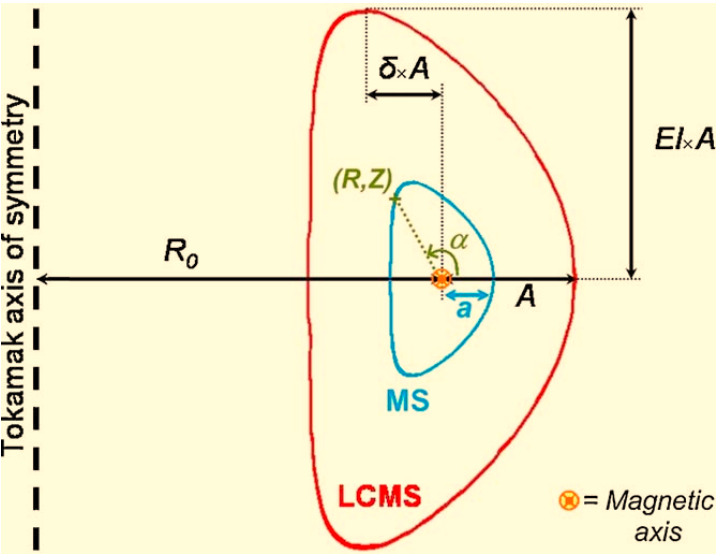
\includegraphics[scale=0.2]{../plots/Analytic_source.png}
  \caption{The analytic source configuration}
  \label{fig:Analytic_source}
\end{figure}

\section{Neutron Wall Loading} \label{Neutron Wall Loading}
The next step in the analysis was applied to the full 3-D model which involved calculations of the NWL distributions at the IB \& OB FWs, the inner \& outer divertor plates, and the middle divertor plate (dome). The vertical distribution of the NWL at the FWs (figure \ref{fig:NWL FWs}) and inner \& outer divertor plates (figure \ref{fig:NWL 2Divs}) were calculated over segments $\sim$ \SI{10}{cm} high starting from the mid-plane and moving upward. It's worth noting that the NWL was calculated at the FW and not over any approximated contour and the segments used in the calculations are shown in figure \ref{fig:NWL segments} for the top half of the model. The radial distribution of the NWL at the dome is shown in figure \ref{fig:NWL Dome}. Table \ref{NWL peak and average values} shows the calculated peak and average values at the FWs and divertors. The average values are area averages over each surface of the corresponding region. The peak values at the FWs occur at the mid-plane while for the inner and outer divertors it occurs at the bottom portion of the plates where it's closer to the plasma source. For the dome the peak value occurs in the middle.  

\begin{figure}[h!]
  \centering
  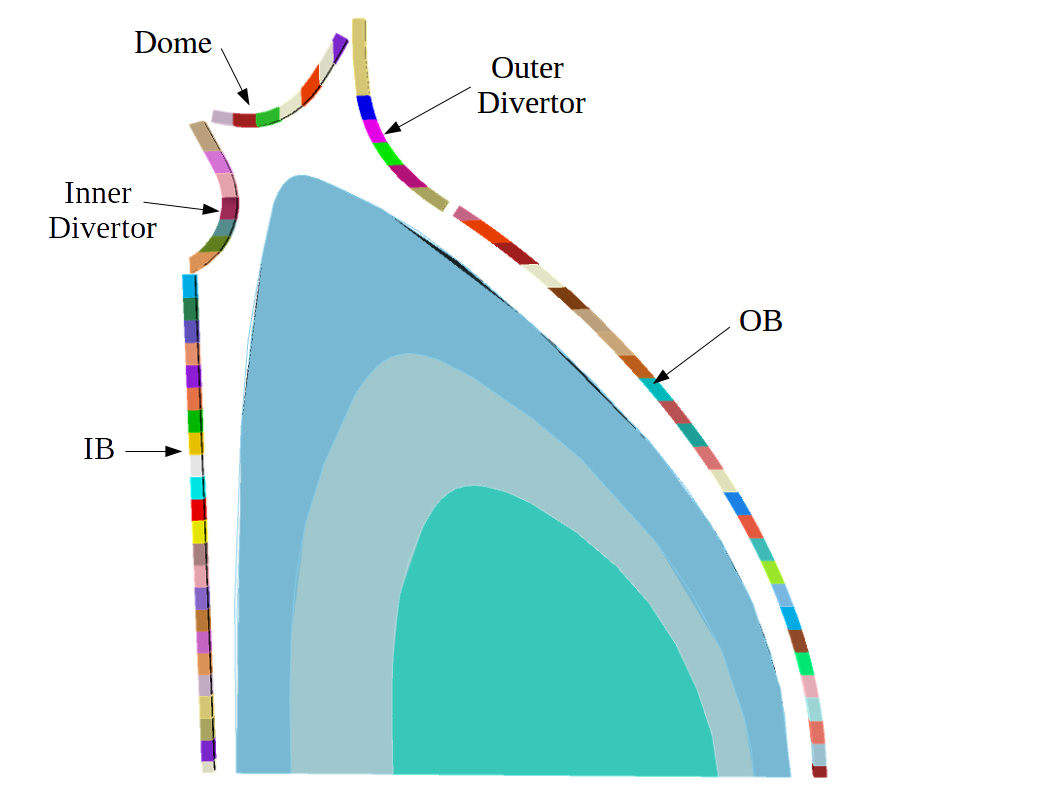
\includegraphics[scale=0.3]{../plots/NWL_segments.png}
  \caption{OB, IB, and Divertor segments used in NWL analysis}
  \label{fig:NWL segments}
\end{figure}
\begin{table}[h!]
	\caption{NWL peak and average values}
	\label{NWL peak and average values}
	\begin{tabular}{ |c|c|c|c| } 
		\hline
		 {} & Peak NWL [MW/m\textsuperscript{2}] & Average NWL [MW/m\textsuperscript{2}] \\
		\hline
		{OB FW} & 1.75 $\pm$ 0.11\% & 1.35 \\
		\hline
		{IB FW} & 1.31 $\pm$ 0.17\% & 0.86 \\
		\hline
		{Inner Divertor} & 0.79 $\pm$ 0.25\% & 0.32 \\
		\hline
		{Dome} & 0.66 $\pm$ 0.27\% & 0.49 \\
		\hline
		{Outer Divertor} & 0.76 $\pm$ 0.14\% & 0.35 \\
		\hline
		{all 3 Divertor plates} & 0.79 $\pm$ 0.13\% & 0.38 \\
		\hline
	\end{tabular}
\end{table}
 \begin{figure}[h!]
  \centering
  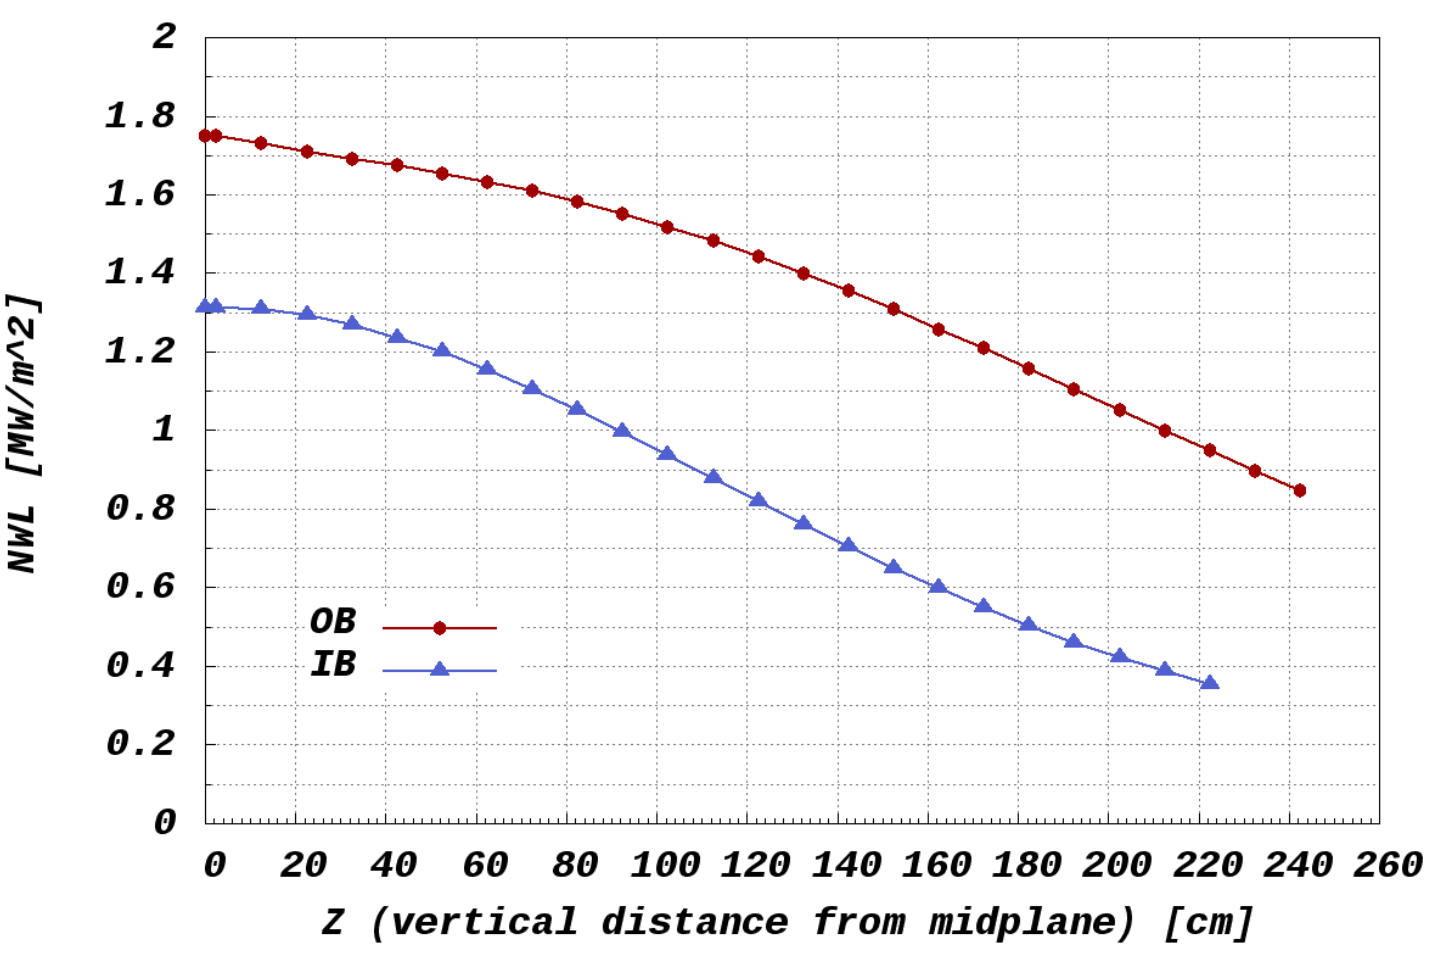
\includegraphics[scale=0.2]{../plots/NWL_FWs.png}
  \caption{The NWL vertical distribution at IB $\&$ OB FW}
  \label{fig:NWL FWs}
\end{figure}
\begin{figure}[h!]
  \centering
  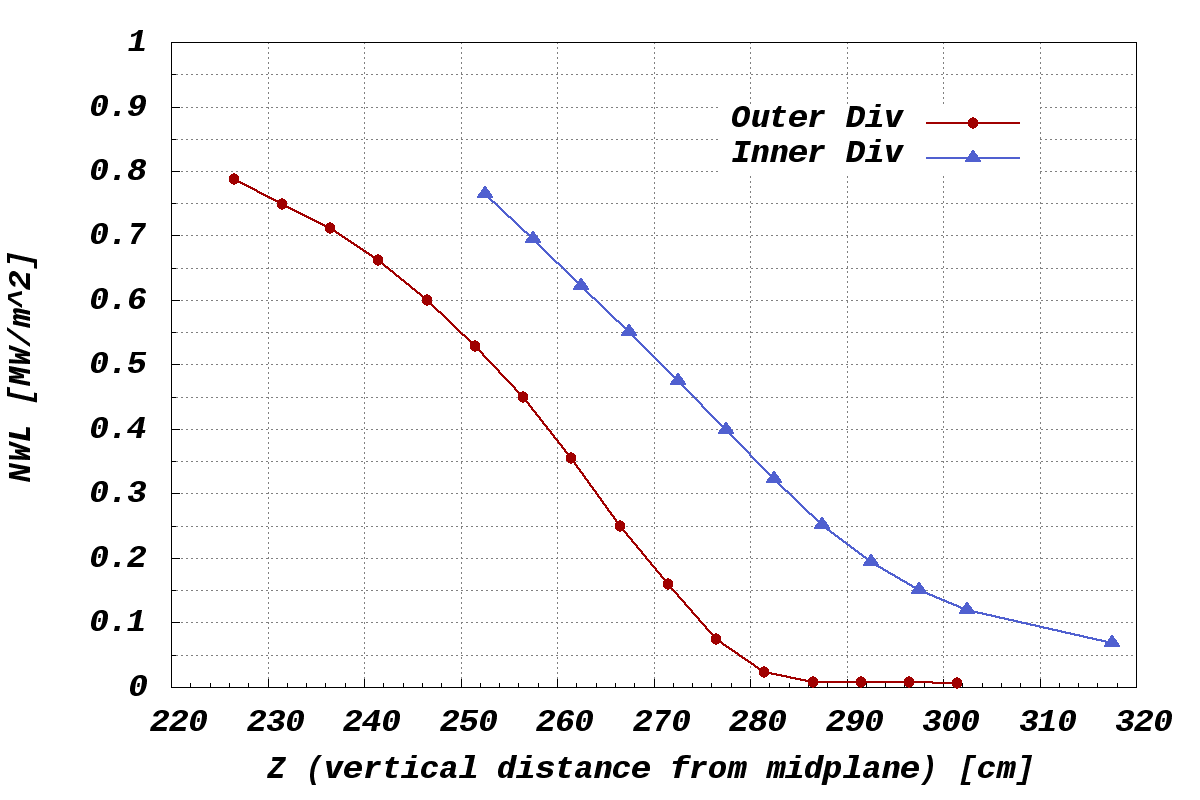
\includegraphics[scale=0.3]{../plots/NWL_2divs.png}
  \caption{The NWL vertical distribution at the inner and outer divertors}
  \label{fig:NWL 2Divs}
\end{figure}
\begin{figure}[h!]
	\centering
	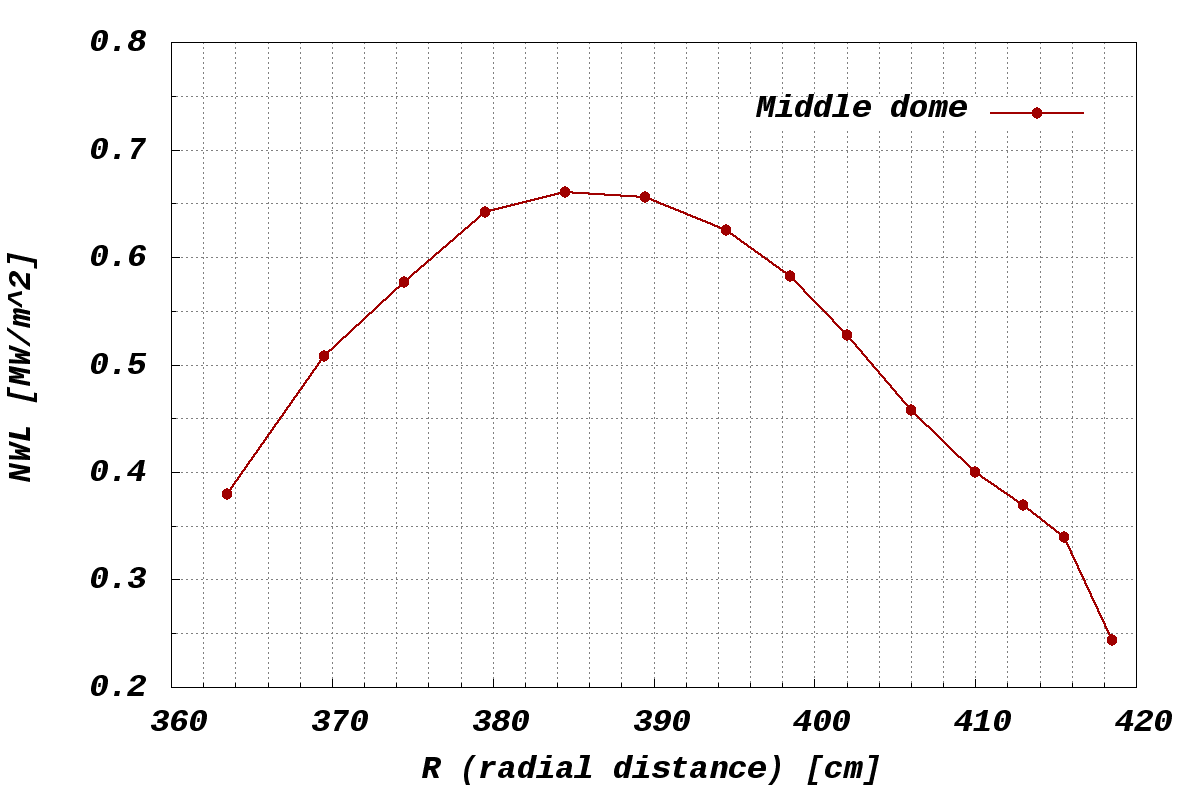
\includegraphics[scale=0.3]{../plots/NWL_div.png}
	\caption{The NWL distribution at the dome}
	\label{fig:NWL Dome}
\end{figure}

\section{Tritium Breeding Calculations} \label{Tritium Breeding Calculations}
The rich fusion research literature shows a growing interest to achieve ignition via the deuterium - tritium (D-T) fuel cycle and due to the scarcity of T in nature and the high cost of T consumed by fusion power plants (55.6 kg/full power year (FPY)/GW\textsubscript{fus}) \cite{ref_3}, all power plants developed to date that employ the D-T fuel cycle are required to breed T in blankets surrounding the plasma. As a result the need for TBR (ratio of tritium bred in the blankets to that consumed in the plasma) calculations with high certainty grew substantially and the TBR is considered an essential metric in the design phase.\vspace{5mm}

The blanket of choice for the FESS-FNSF project is the dual cooled lead-lithium (DCLL) \cite{ref_12} blanket. The blanket consists of $\sim$ \SI{20}{cm} radial/toroidal flow channels of LiPb eutectic (15.7 at\% Li (90\% Li$^6$ enrichment) and 84.3 at\% Pb) surrounded by \SI{0.5}{cm} SiC FCI (flow channel insert) and \SI{0.2}{cm} layer of LiPb. The blanket structure is cooled by helium at high pressure (\SI{8}{MPa}) which is also used for heat removal in other components such as FW and blanket side/back/front walls. The blanket also serves other purposes besides breeding T such as the removal of volumetric heat deposited by fast neutrons from the plasma and shielding the outer components such as the structural ring (SR), the vacuum vessel (VV), and the magnets.

\subsection{TBR Workflow} \label{TBR Workflow}
Using the previously established workflow to estimate incremental effects of
geometry on the TBR from \cite{ref_13}, the calculation
of the TBR was performed. The workflow
consists of a multi-step approach to calculate the TBR by starting the analysis
with a CAD model with a simplified breeding blanket and at each step a new
detail is added such as the He flow channels, the side walls, etc. and the
resulting TBR of the facility is calculated at each step. The TBR results are
shown in figure \ref{fig:TBR chart}. \vspace{5mm}

Step 1 is a reference case showing the TBR for an infinite cylinder of LiPb surrounded by shields with a coaxial plasma source. The calculated value represents the maximum achievable TBR for a hypothetical infinite medium. In step 2, the model was constructed of 16 sectors each consisting of IB and OB breeding blankets surrounded by shields and divertors with \SI{2}{cm} assembly gaps between the sectors. The 3-D configuration with such radial and poloidal coverage (compared to the infinite case in step 1) resulted in a TBR drop of 19.74\%. The assignment of the homogenized composition (34\% ferritic steel (FS), 66\% He) to the \SI{3.8}{cm} thick IB and OB FWs in all sectors (step 3) resulted in a TBR drop of 8.7\%. Modelling of side walls (same thickness and composition as FW) and the \SI{2}{cm} thick back walls (80\% FS, 20\% He) in all sectors (step 4) resulted in an additional TBR drop of 2.79\%. Defining the main LiPb flow channels by modelling the \SI{1.5}{cm} cooling channels with an assigned composition (58\% FS, 42\% He) in all sectors (step 5) resulted in a further drop of 3.95\%. Assigning 34\% SiC to the \SI{0.5}{cm} FCI in all sectors (step 6) resulted in a drop of 4.6\%. Adding the \SI{2}{cm} IB and OB stabilizing shells (W alloy) to all sectors (step 7) resulted in a drop of 4.11\%.
\begin{figure}[h!]
  \centering
  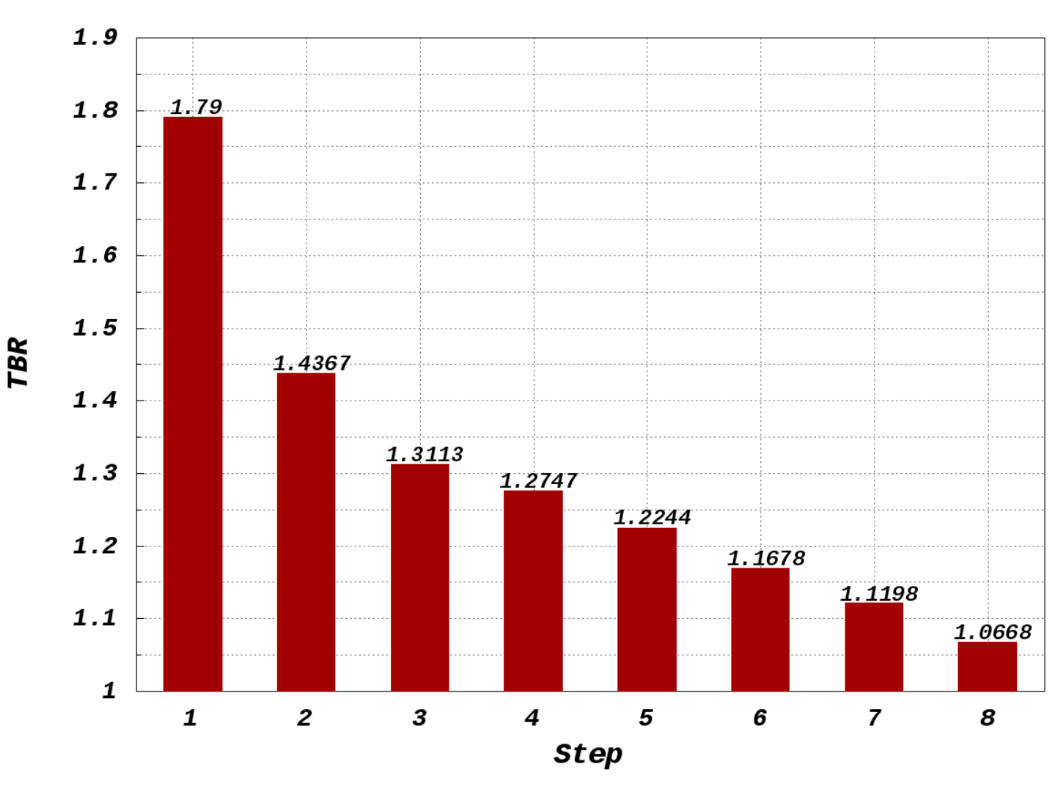
\includegraphics[scale=0.3]{../plots/TBR_chart.png}
  \caption{TBR chart}
  \label{fig:TBR chart}
\end{figure}

\subsection{Penetrations and Ports} \label{Penetrations and Ports}
The facility has 12 mid-plane and 6 off-mid-plane ports, the effect of which was assessed by adding each type of ports to the respective sectors (for analysis purposes) and calculate the facility overall TBR and the corresponding drop (compared to step 7). It's worth noting that the ports were modelled in detail; frames, gaps, blanket frames, and internal structures were included in the CAD model. Adding the material testing module (MTM) to 1 sector (\SI{1}{m\textsuperscript{2}} at FW) resulted in a drop of 0.313\%. The facility has 4 testing blanket modules (TBM) (in 4 sectors, \SI{1}{m\textsuperscript{2}} each at FW), for purposes of testing different breeding concepts, resulting (all four TBMs) in a drop in the TBR of 0.2\%. The three plasma diagnostics ports resulted in a drop of 0.95\%. Including two neutral beam injectors (NBI) (in 4 sectors, \SI{1.9}{m\textsuperscript{2}} each at FW) reduced the TBR by 1.63\%. \vspace{5mm}

The remaining ports; IC (in 1 sector, \SI{2}{m\textsuperscript{2}} at FW), LH (in 1 sector, \SI{1.5}{m\textsuperscript{2}} at FW), EC (in 1 sector, \SI{0.675}{m\textsuperscript{2}} at FW), Fueling (in 1 sector, \SI{0.04}{m\textsuperscript{2}} at FW), Disruption mitigation (in 1 sector, \SI{0.04}{m\textsuperscript{2}} at FW), and two Divertor diagnostics (in 1 sector, \SI{0.15}{m\textsuperscript{2}} each at FW) resulted in a TBR drop of 0.71\%, 0.5\%, 0.23\%, 0.02\%, 0.02\%, and 0.08\%, respectively. A final step (step 8 on figure \ref{fig:TBR chart}) with all penetrations included at the same time resulted in a drop of 4.95\%. A planar cross section of the facility with all penetrations identified is shown in figure \ref{fig:Ports}.
\begin{figure}[h!]
  \centering
  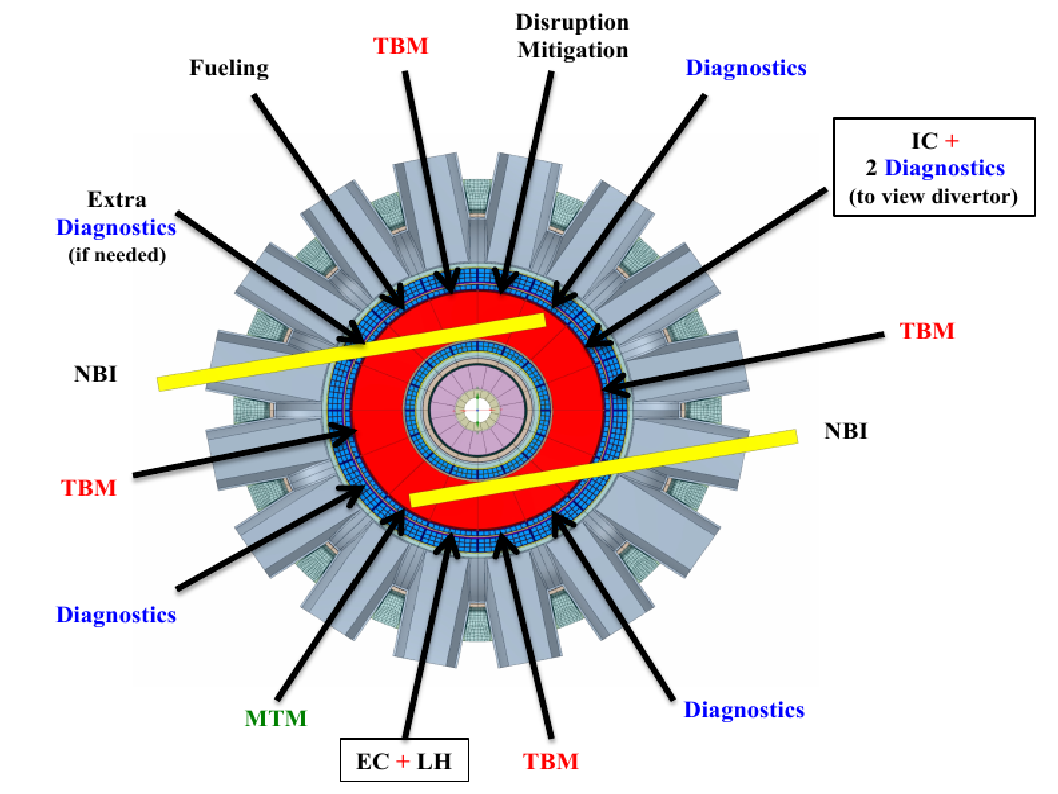
\includegraphics[scale=0.3]{../plots/ports.png}
  \caption{Cross-section of the facility at the mid-plane}
  \label{fig:Ports}
\end{figure}

\subsection{Li-6 Enrichment} \label{Li-6 Enrichment}
One of the advantages of the DCLL blanket is allowing the control of the T bred by controlling the  Li\textsuperscript{6} enrichment in LiPb in the main flow channels. Controlling Li\textsuperscript{6} enrichment is necessary to avoid dealing with a surplus or shortage of T. Analyses were performed to test the effect of changing Li\textsuperscript{6} enrichment on the overall TBR of the facility (with all penetrations and ports included) and it was found that the TBR dropped to $1.0191\pm 0.03\%$, $0.9892\pm 0.03\%$, and $0.9513\pm 0.03\%$ for 70\%, 60\%, and 50\% Li\textsuperscript{6} enrichment, respectively. The TBR satisfies the tritium breeding requirement of 1.04 with ~ 80\% Li\textsuperscript{6} enrichment and the results are shown in figure \ref{fig:Li6_enrichment}.
\begin{figure}[h!]
  \centering
  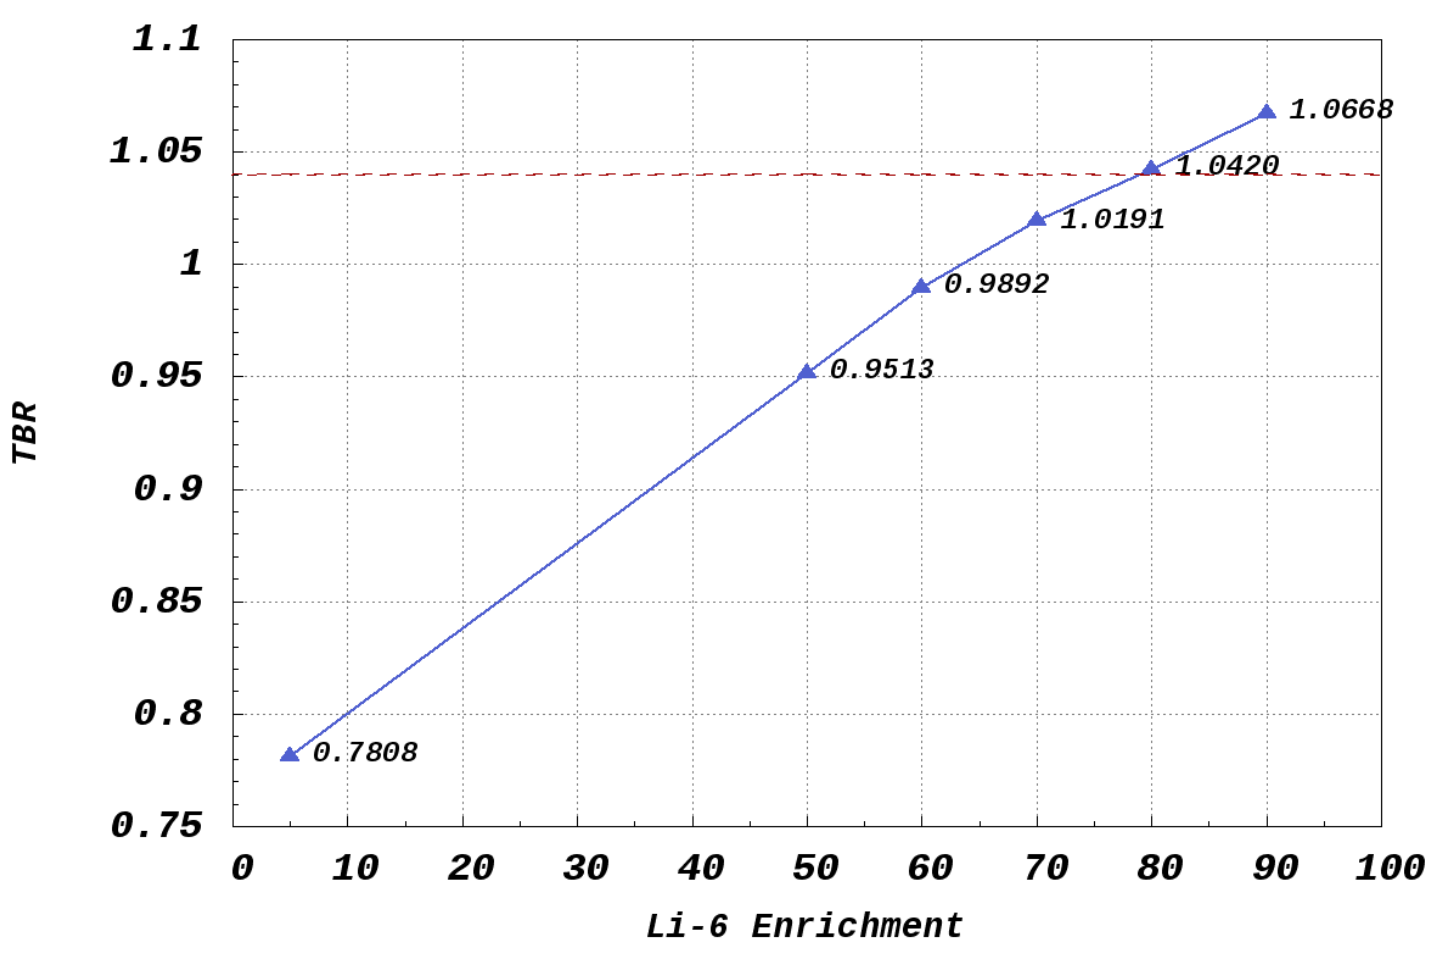
\includegraphics[scale=0.2]{../plots/Li6_enrichment.png}
  \caption{The facility overall TBR vs Li6 enrichment}
  \label{fig:Li6_enrichment}
\end{figure}

\subsection{TBR mapping} \label{TBR mapping}
One of the concepts implemented in the current design – based on experience with previous models – is keeping the mid-plane clear of any ports or penetrations as practically achievable. The current model has a peak NWL of 1.75 and \SI{1.31}{MW/m\textsuperscript{2}} at the OB and IB mid-planes, respectively. This could directly be related to the calculated TBR (74\% OB and 26\% IB yield) showing that more T is produced near the mid-plane compared to the upper and lower (poloidal direction) or back (radial direction) of both the \SI{0.5}{m} IB and the \SI{1}{m} OB blankets.\vspace{5mm}

Using DAG-MCNP5 mesh tally capabilities the T production was mapped in the IB and OB blankets of one sector as shown in figure \ref{fig:step7} for step 7 and figure \ref{fig:NBI} for the NBI. Figure \ref{fig:step7} also shows a reduction in TBR behind the stabilizing shells due to the absorption of neutrons by W. Including any penetrations in the mid-plane will have an effect on the overall TBR by reducing the active volume of the blanket where it's most effective for T breeding, even though there may be slightly enhanced local T breeding far inside the blanket due to streaming of neutrons.
\begin{figure}[h!]
\centering
\begin{subfigure}{0.49\textwidth}
  \centering
  \includegraphics[width = \textwidth]{../plots/step7_clip.png}
  \caption{Sector without any ports}
  \label{fig:step7}
\end{subfigure}
\begin{subfigure}{0.49\textwidth}
  \centering
  \includegraphics[width = \textwidth]{../plots/NBI_clip.png}
  \caption{Sector with NBI}
  \label{fig:NBI}
\end{subfigure}
\caption{Mapping of the tritium production in two different sectors}
\label{fig:TBR mapping}
\end{figure}

\section{Radiation Damage} \label{Radiation Damage}
The shielding analysis followed the tritium breeding blanket optimisation to provide the needed protection of the lifetime components. The main shielding design philosophy (as employed in previous designs \cite{ref_14}) is that every layer provides protection to the following layers such that collectively they would protect the out-of-vessel components such as the magnets. For example, in addition to the T breeding, the blanket (both the IB and OB) is supposed to provide protection for the structural ring and in turn both would protect the vacuum vessel and finally all three layers would attenuate the neutron and gamma fluxes to such low levels to protect the magnets. Such an approach requires some trade offs between compactness and performance to identify the optimal composition. An example would be the optimisation of the VV, SR, and LT shield; the need for a compact IB radial build suggested the use of the WC filler for the SR, VV, and LT shield to reduce the major radius of the facility while the B-FS filler is limited to the OB and top/bottom sections of the SR and LT shield. Shown in figure \ref{fig:flux mapping} is a mapping of the neutron flux in the facility at the mid-plane (z=0) and from the figure it can be seen that a reduction of three orders of magnitude of the neutron flux across the OB breeding zone and SR is achieved. A detailed discussion of shielding optimisation can be found in \cite{ref_2}. 
\begin{figure}[h!]
	\centering
	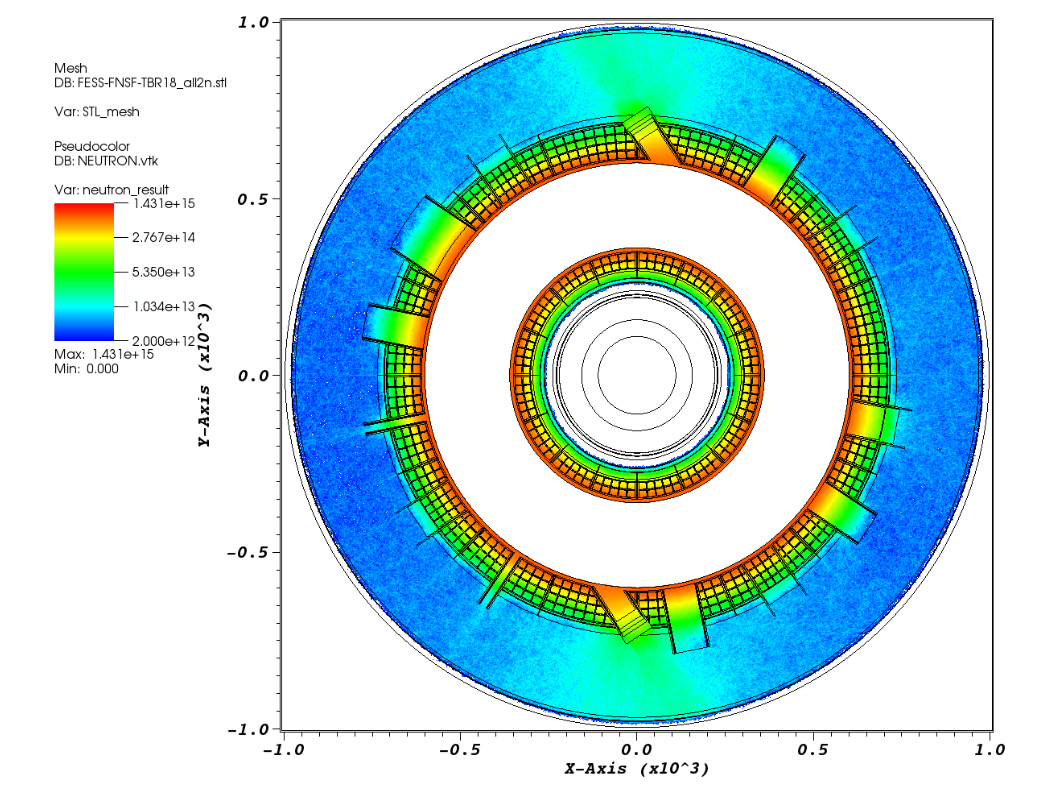
\includegraphics[scale=0.4]{../plots/flux.png}
	\caption{Mapping of the neutron flux at the mid-plane (z=0)}
	\label{fig:flux mapping}
\end{figure}

\subsection{dpa, He/H production} \label{dpa, He/H production}
The damage caused by irradiation to the in-vessel components is an important factor in the selection of materials in the design phase. The radiation damage can be quantified using two main parameters: displacement per atom (dpa) and gas (He and H) production. These parameters impact the lifetime of structural components and the potential for reweldability after irradiation.\vspace{5mm}

For the FW, the peak values calculated at the mid-plane are shown in table \ref{Radiation damage values for the FW and VV}. The radial distribution of the damage to the ferritic steel alloy (F82H) is shown in figure \ref{fig:Radial Damage}. It's worth noting that there is a slight increase in the He and H production near the end of the blanket at \SI{700}{cm} due to the strong neutron reflection from the SR/VV/shield. The reweldability of the VV is directly related to the levels of H and He produced during the operation and that leads to setting a limit of \SI{1}{He\hspace{1 mm} appm} which shouldn't be exceeded at any time during plant operation. An issue that needs to be addressed is the streaming through the assembly gaps (\SI{2}{cm} between the OB and IB sectors) and all penetrations described in section \ref{Penetrations and Ports} which will cause peaking in radiation damage to the exposed portions of the VV. The results of the damage at the VV mid-plane (away from the NBIs) are listed in table \ref{Radiation damage values for the FW and VV}.   
\begin{table}[h!]
	\caption{Radiation damage values for the FW and VV}
	\label{Radiation damage values for the FW and VV}
	\begin{tabular}{ |c|c|c|c|c| } 
		\hline
		{} & \multicolumn{2}{|c|}{FW} & \multicolumn{2}{|c|}{VV} \\
		\hline
		{} & IB & OB & IB & OB \\
		\hline
		\multirow{2}{6em}{Damage [dpa/FPY]} & 13.70 $\pm$ 1.53\% & 15.25 $\pm$ 0.92\% & 0.1495 $\pm$ 0.64\% & 0.0114 $\pm$ 0.36\%  \\
		& {} & {} & {} & {} \\
		\hline
		\multirow{2}{6em}{He [appm/FPY]} & 137.30 $\pm$ 2.52\% & 154.58 $\pm$ 1.41\% & 0.3109 $\pm$ 8.83\% & 0.0029 $\pm$ 13.81\%  \\
		& {} & {} & {} & {} \\
		\hline
		\multirow{2}{6em}{He/dpa ratio} & 10.02 & 10.14 & 2.08 & 0.26  \\
		& {} & {} & {} & {} \\
		\hline
		\multirow{2}{6em}{H [appm/FPY]} & 613.50 $\pm$ 2.42\% & 691.94 $\pm$ 1.35\% & 0.2462 $\pm$ 8.92\% & 0.0025 $\pm$ 12.99\%  \\
		& {} & {} & {} & {} \\
		\hline
	\end{tabular}
\end{table}
\begin{figure}[h!]
  \centering
  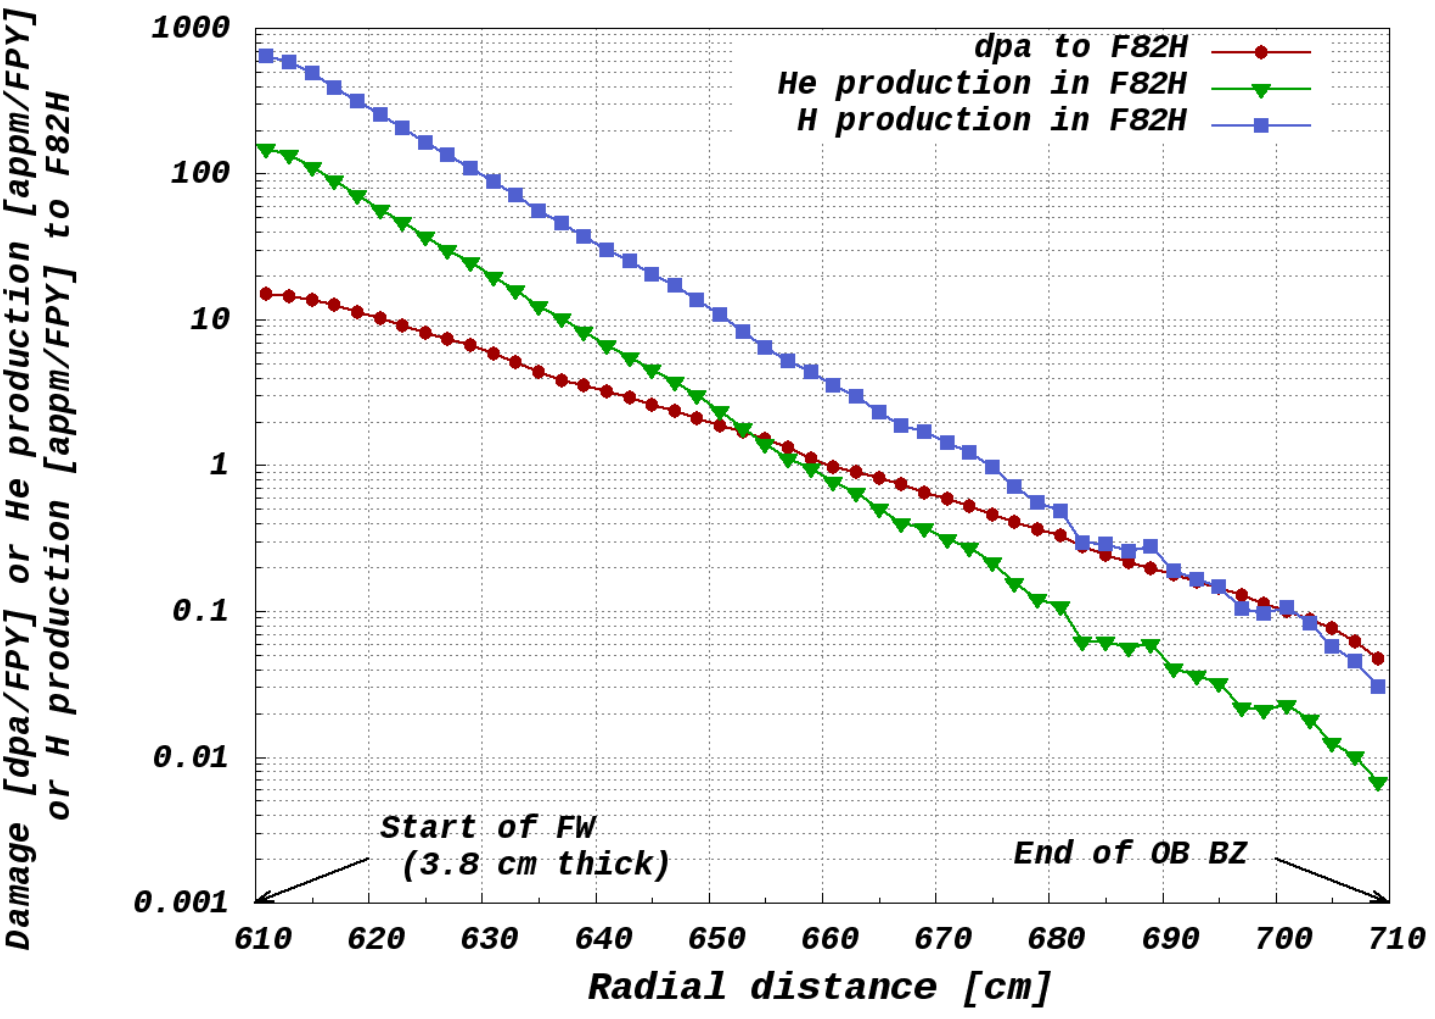
\includegraphics[scale=0.2]{../plots/radialdamage.png}
  \caption{The radial distribution of radiation damage at OB}
  \label{fig:Radial Damage}
\end{figure}

\subsection{Magnet damage} \label{Magnet damage}
\providecommand{\e}[1]{\ensuremath{\times 10^{#1}}}
The magnet is a critical component of the facility and is considered the main focus of all shielding optimisation efforts. Following the shield design philosophy stated previously, the 3-D neutronics analysis confirmed that the radiation levels at the magnet winding pack (WP) met the limits set by the magnet designers. Calculations showed that the peak fast (E $>$ \SI{0.1}{MeV}) neutron fluence at the WP 1.35\e{18} $\pm$ 4.58\% n/cm\textsuperscript{2} is well below the limit (5\e{18} n/cm\textsuperscript{2}). The LT shield behind the VV has WC (37\%) and H2O (33\%) which combined have superior shielding capacity in attenuating the neutron flux. The peak nuclear heating at the coil case “CC” is 0.26 $\pm$ 2.55\% mW/cm\textsuperscript{3}, below the limit of \SI{2}{mW/cm\textsuperscript{3}}. The peak dpa to the Cu stabilizer is 9.54\e{-5} $\pm$ 4.1\% dpa/FPY, also below the limit of 10\e{-4} dpa/FPY. The peak dose to the electrical insulator was also calculated and found to be 5.25\e{8} $\pm$ 4.91\% rads.

\subsection{Total Heating}
The total heating (neutron and gamma) was calculated for the model without any penetrations or ports inserted making use of the symmetry of all 16 sectors. Using DAG-MCNP5 the total heating tallies (F6) were calculated for all sub-volumes in one sector and the results were divided into 7 categories as shown in table \ref{np_heating}. The regions are color-coded in figure \ref{fig:Heating regions} with the corresponding titles as appear on the table. The OB result is a sum of the heating over all regions from the FW up to the SR; OB FW, SW, BW, cooling channel, LiPb flow channels, liners, stabilizing shells, He manifold, and kink shell. The IB result is a sum over the corresponding regions on the IB; IB FW, SW, BW, cooling channel, LiPb flow channels, liners, stabilizing shells, and He manifold. The heating was calculated for the three divertor plates both the top and bottom and the sum is given in the table and similarly for the dome shield and the box enclosing the divertors. \vspace{5mm}

The total nuclear heating results for the stabilizing shells on the OB and IB are 0.8017 $\pm$ 0.4\% and 0.055 $\pm$ 1.4\% MW respectively. The total nuclear heating in all regions in the facility (all 16 sectors) = \SI{475.7}{MW} which results in an energy multiplication factor (ratio of source neutron energy to total heating) of 1.15. 
\begin{table}[h!]
	\caption{Total (n+p) heating in all regions}
	\label{np_heating}
	\centering
	\begin{tabular}{ |c|c|c|c| }
		\hline
		 {} & Neutron Heating [MW] & Gamma Heating [MW] & Total [MW] \\
		\hline
		{Strucutral Ring "SR"} & 0.41 $\pm$ 0.18\% & 0.99 $\pm$ 0.42\% & 1.40 $\pm$ 0.30\% \\
		\hline
		{Divertor shield and Box} & 0.21 $\pm$ 0.31\% & 0.98 $\pm$ 0.43\% & 1.19 $\pm$ 0.36\% \\
		\hline
		{Divertor plates} & 0.09 $\pm$ 0.28\% & 1.75 $\pm$ 0.31\% & 1.84 $\pm$ 0.29\% \\
		\hline
		{Vacuum Vessel "VV"} & 0.03 $\pm$ 0.07\% & 0.15 $\pm$ 0.25\% & 0.18 $\pm$ 0.21\% \\
		\hline
		{LT shield} & 0.18 $\pm$ 0.06\% & 0.12 $\pm$ 0.25\% & 0.31 $\pm$ 0.11\% \\
		\hline
		{IB} & 3.51 $\pm$ 0.14\% & 2.83 $\pm$ 0.28\% & 6.34 $\pm$ 0.15\% \\
		\hline
		{OB} & 9.95 $\pm$ 0.10\% & 9.03 $\pm$ 0.17\% & 18.98 $\pm$ 0.10\% \\
		\hline
	\end{tabular}
\end{table}
\begin{figure}[h!]
  \centering
  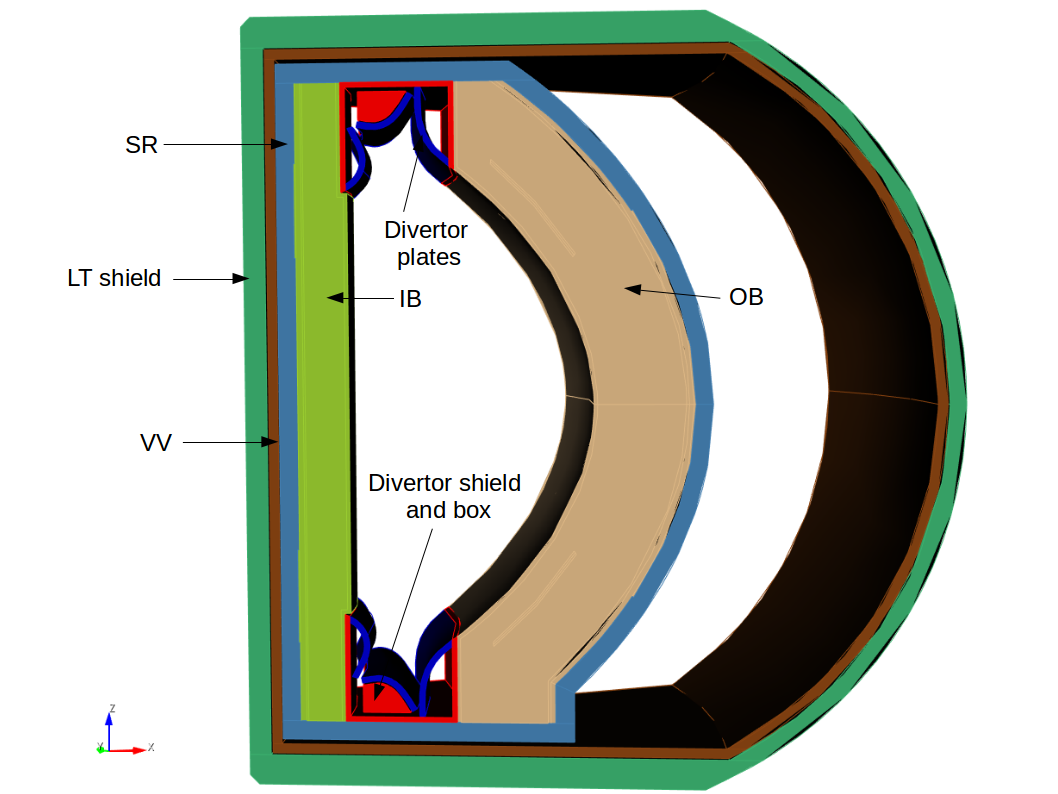
\includegraphics[scale=0.4]{../plots/heating_regions.png}
  \caption{Definition of heating regions tabulated in table 3}
  \label{fig:Heating regions}
\end{figure}

% \section{Shutdown Dose Rate Calculations} \label{Shutdown Dose Rate Calculations}
% Part of the design effort of next step machines like the FESS-FNSF is dedicated to maintenance. The current design allows moving each sector of the 16 sectors individually through designed ports for purposes of maintenance or repair of components. An important question that needs to be aswered during the analysis phase of the design is the wait time after shutdown of the machine till the radiation levels are dropped below the allowed limits for personal access or handling outside the shield. To achieve such task, the calculation of the shutdown dose rate with high certainty, state-of-the-art tools were used. DAG-MCNP5 was used for photon transport and the activation code ALARA was used for nuclides inventory analysis and calculation of decay gamma source distribution.\vspace{5mm}   

% \subsection{Workflow} \label{SDR_workflow}
% The shutdown dose rate is due to decay photons emitted by radioactive nuclides generated during operation from neutron interactions. The calculation of shutdown dose rate is achieved following three main steps; 1) Neutron transport calculation, 2) Nuclide inventory calculation, and 3) Decay gamma transport calculations.\vspace{5mm}

% Step (1) involved neutron transport calculation on the facility without any ports or penetrations inserted which is believed to produce an upper bound for the radiation levels due to the fact that insertion of ports remove parts of the active volume of sectors leading to streaming to the outer VV and LT shield. Using meshtally capabiities of DAG-MCNP5 the spatial distribution of the neutron flux on a \SI{6x6x6}{cm} mesh covering one sector of the 16 sectors was calculated. In step (2) the activation inventories and decay gamma sources (spectrum and intensity) were calculated for all regions in the sector using the corresponding materials along with the associated neutron flux spectra obtained in step (1). A simplified irradiation scenario was used; \SI{0}{s}, \SI{1}{d}, \SI{2}{d}, \SI{7}{d}, \SI{14}{d}, \SI{0.1}{y}, and \SI{0.25}{y}.\vspace{5mm}

% The produced distribution of the decay gamma intensities in the mesh from step (2) is then used to produce the photon source distribution using the r2s module from the PyNE toolkit. The module produces a source file for each time step of the irradiation scenario which is then used for photon transport on the sector using DAG-MCNP5 totalling 7 calculations. Also for the purpose of clculating the temperature rise due to the desipated energy in the sector the heating due to the decay gamma energy deposition was calculated for each time step in the irradiation scenario. \vspace{5mm}

% \subsection{SDR: results} \label{SDR}


% \subsection{Decay Heat: results} \label{Decay Heat}
% Table \ref{photon heating} gives the results of decay gamma heating in one sector at different times following the shutdown of the facility. The source strength at each time step was calculated using ALARA.

% \begin{table}[h!]
% 	\caption{Photon heating following shutdown}
% 	\label{photon heating}
% 	\begin{tabular}{ |c|c|c|c| } 
% 		\hline
% 		Time step & Decay gamma source intensity [p/s] & Photon heating [MW] \\
% 		\hline
% 		{\SI{0}{s}} & 5.52\e{19} & 4.100 $\pm$ 0.04\% \\
% 		\hline
% 		{\SI{1}{d}} & 1.52\e{19} & 0.777 $\pm$ 0.07\% \\
% 		\hline
% 		{\SI{2}{d}} & 9.28\e{18} & 0.461 $\pm$ 0.06\% \\
% 		\hline
% 		{\SI{7}{d}} & 3.47\e{18} & 0.159 $\pm$ 0.05\% \\
% 		\hline
% 		{\SI{14}{d}} & 3.01\e{18} & 0.141 $\pm$ 0.05\% \\
% 		\hline
% 		{\SI{0.1}{y}} & 2.67\e{18} & 0.131 $\pm$ 0.05\% \\
% 		\hline
% 		{\SI{0.25}{y}} & 2.28\e{18} & 0.109 $\pm$ 0.05\% \\
% 		\hline
% 	\end{tabular}
% \end{table}

\section{Conclusions} \label{conclusion}
The analysis contained within this paper demonstrates some of the key nuclear parameters that help define the nuclear environment within the test facility. Specifically with regards to TBR the individual worth of each sector was determined, the ultimate impact on TBR scaled well with the cross sectional area, with 
the exception of the TBMs since they are a source of tritium. Furthermore, for the nominal baseline design it was determined that the FNSF can be self sufficient in terms of tritium production if the lithium is enriched to 80 at\%. Peak DPA rates were found to be 15 DPA/FPY, helium production was found to peak at 155 appm  and hydrogen production was found to be 692 appm, all peaking at the OB FW. The damage and heating to the winding pack of the IB magnets were all found to be below the limits specified. There are a number of differences between this FNSF and a full power reactor; the neutron wall loading is projected to be higher in full power plant by a factor of $\sim$ 2 resulting in higher neutron fluxes at the FW, the damage \& gas production rates will similarly be proportionally higher, however these parameters scale linearly with the fusion power. There are also a number of similarities with future plants; the helium production rate /dpa rate ratio will be similar, and neutron transmutation rates will also be similar.
\\

%The fusion community has benefited from the wealth of fission based nuclear data that exists, however certainly for transmutation cross sections there can be significant uncertainty in the neutron cross section data, thus a suite of experiments should be planned that determine the key cross sections to an accuracy as required by analyses. The best suite of neutron induced reaction data are currently the TENDL \cite{ref_15} data, effort should be made to ensure the neutron transmutation codes used can support this data. Currently, the best estimates of the uncertainty \cite{ref_16} in the $^6$Li \& $^7$Li (n,t) pathways are often very close to the excess tritium produced in the design, effort should therefore be undertaken to determine these cross sections to a much lower uncertainty.
%This is particularly critical since for several fusion power plant designs there is very little 
%\\
%
%Future work should also focus on the development of a coupled analysis amongst all physical modelling that has feedback to the neutronics calculation. Such a coupling would allow the proper coupling of neutronics, thermo-mechanical, magnetic, and other detailed physics to properly account for material and geometric changes that impact the modelling of fusion systems. A prescient example would be the determination of all heat loads onto a component, how the resultant heat source impacts the thermo-mechanical behaviour of the system, and then determining the impact of those structural changes to the neutronics of the system.

\newpage
\section{References}
\begin{thebibliography}{14} 
\bibitem{ref_1} 
C. E. KESSEL, et al., {“The Fusion Nuclear Science Facility, the Critical Step in the Pathway to Fusion Energy,” Fusion Science and Technology, vol. 68, p. 225–236 (2015).}
\bibitem{ref_2} 
  L. El-Guebaly, et al., {“Design Approach for FESS-FNSF In-Vessel Components and Constraints Imposed on Radial/Vertical Build Definition,” presented at 22nd ANS Topical Meeting on the Technology of Fusion Energy (TOFE), August 22 -25, 2016, Philadelphia, PA}
\bibitem{ref_3}
L. A. EL-GUEBALY, et al., {“Toward the Ultimate Goal of Tritium Self-Sufficiency: Technical Issues and Requirements Imposed on ARIES Advanced Power Plants,” Fusion Engineering and Design, vol. 84, p. 2072-2083 (2009).}
\bibitem{ref_4}
X-5 Monte Carlo Team, {MCNP a General Monte Carlo N-Particle Transport Code Version 5, Tech. Rep. LA-CP-03-0245, Los Alamos National Laboratory, MCNP 5, (March 2005).}
\bibitem{ref_5}
{DAGMC: http://svalinn.github.io/DAGMC/}
\bibitem{ref_6}
{PyNE: http://pyne.io/} 
\bibitem{ref_7}
D. L. ALDAMA and et al., {“FENDL2.1, Update of an Evaluated Nuclear Data Library for Fusion applications.” IAEA report INDC (NDS) 467, Vienna, Austria (2004).}
\bibitem{ref_11}
Clement Fausser, et al., {“Tokamak D-T Neutron Source Models for Different Plasma Physics Confinement Modes.” Fusion Engineering and Design, vol. 87, p. 787–792 (2012).}
\bibitem{ref_12}
S. MALANG et al., {“Development of the Lead Lithium (DCLL) Blanket Concept,” Fusion Science and Technology, 60, 249 (2011).}
\bibitem{ref_13}
  L El-Guebaly, A Jaber, L Mynsberge, et al, {"State-of-the-Art 3-D Assessment of Elements Degrading TBR of ARIES-ACT SiC/LiPb Blanket," Fusion Science and Technology 64 (3), 582 (2013).}
\bibitem{ref_14}
  L. EL-GUEBALY and the ARIES Team, {“Overview of ARIES-RS Neutronics and Radiation Shielding: Key Issues and Main Conclusions,” Fusion Engineering and Design, vol. 38, p. 139 – 158 (1997).}
%\bibitem{ref_14}
%L. EL-GUEBALY and the ARIES Team, {“Overview of ARIES-RS Neutronics and Radiation Shielding: Key Issues and Main Conclusions,” Fusion Engineering and Design, vol. 38, p. 139 – 158 (1997).}
\bibitem{ref_15}
A.J. Koning, D. Rochman, J. Kopecky, J. Ch. Sublet, E. Bauge, S. Hilaire, P. Romain, B. Morillon, H. Duarte, S. van der Marck, S. Pomp, H. Sjostrand, R. Forrest, H. Henriksson, O. Cabellos, S. Goriely J. Leppanen, H. Leeb, A. Plompen and R. Mills, {"TENDL-2015: TALYS-based evaluated nuclear data library",  https://tendl.web.psi.ch/tendl\_2015/tendl2015.html}
\bibitem{ref_16}
P. Batistoni et al., {{"Neutronics experiments for uncertainty assessment of tritium breeding in HCPB and HCLL blanket mock-ups irradiated with 14 MeV neutrons"},Nuclear Fusion, 52, 8, 083014}
\end{thebibliography}
\end{document}
